\FloatBarrier
Para a simulação da solução clássica da Segunda Lei de Fick (Seção \ref{sec:sol-numerica-2alei}), foram utilizados 
os parâmetros da Tabela \ref{tab:resumoParametros} e a concentração de equilíbrio obtida na Seção \ref{sec:ceq-param}. Os valores de $\Delta t$ e $\Delta x$ utilizados foram 0,01s e 0,1 $\mu m$, para um tempo total de 22 horas e 35 $\mu m$ de profundidade, com temperatura igual a 718K.

As Figuras \ref{fig:fick-cscte} e \ref{fig:fick-cscte2} mostram o perfil de concentração de nitrogênio obtido para alguns intervalos de tempo ao longo da simulação.

\begin{figure}[ht]
\centering
	\caption{Resultado da simulação da Segunda Lei de Fick para concentração na superfície constante, até 2 horas}
	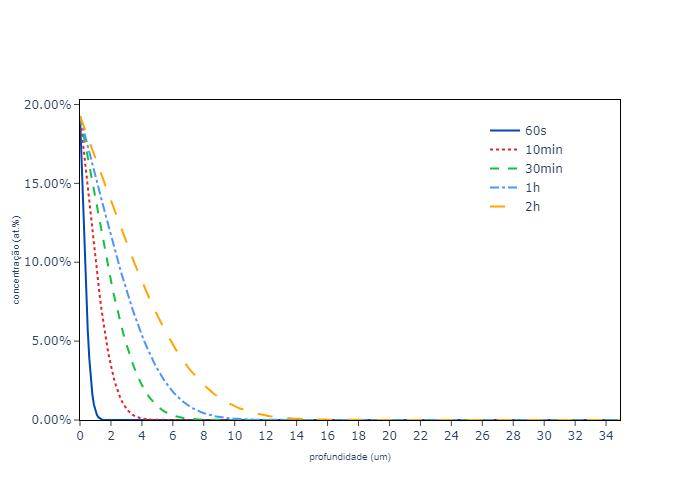
\includegraphics[width=1.0\textwidth]{plot_fickCte1}
	\label{fig:fick-cscte}
	\centering
	\fonte{Elaborado pela autora}
\end{figure}


\begin{figure}[ht]
\centering
	\caption{Resultado da simulação da Segunda Lei de Fick para concentração na superfície constante, até 22 horas}
	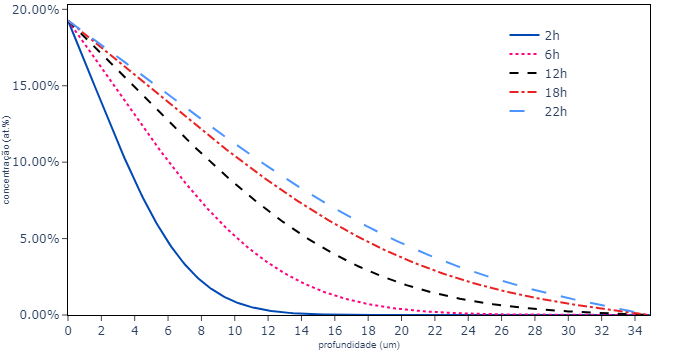
\includegraphics[width=1.0\textwidth]{plot_fickCte2}
	\label{fig:fick-cscte2}
	\centering
	\fonte{Elaborado pela autora}
\end{figure}

\FloatBarrier